\documentclass[journal=jctcce,manuscript=article]{achemso}
\usepackage[T1]{fontenc}
\usepackage{microtype,graphicx,amsmath,amssymb,booktabs,tabularx,siunitx}
\graphicspath{{../figures/main/}{../figures/si/}}
\title{When Does CO$_2$/N$_2$ Selectivity Emerge in Metal--Organic Frameworks?}
\author{Hosein Alimardani}\affiliation{Faculty of Engineering, University of Tehran, Tehran, Iran}
\author{Angelo Di Bella}\affiliation{Lucy Cavendish College, University of Cambridge, Cambridge, United Kingdom}
\author{Shayan Abaei}\affiliation{Department of Chemical Engineering, Faculty of Engineering, University of Tehran, Tehran, Iran}
\author{Uzair Abdullah}\affiliation{Lucy Cavendish College, University of Cambridge, Cambridge, United Kingdom}
\author{Miguel Jorge}\affiliation{Department of Chemical Engineering, University of Strathclyde, Glasgow, United Kingdom}
\author{Mehrdad Asgari}\affiliation{Lucy Cavendish College, University of Cambridge, Cambridge, United Kingdom}
\email{asgarimehrdad89@gmail.com}
\begin{document}

\begin{abstract}
Henry-law selectivity indicates whether a metal--organic framework (MOF) favors CO$_2$ over N$_2$ at infinite dilution, but does not identify the interactions that create this preference. We compare 238 MOFs at 298~K using three nested molecular models: a repulsive Weeks--Chandler--Andersen reference, complete Lennard--Jones interactions without charges, and the charged full potential. All repulsive-reference point estimates favor N$_2$, whereas restoring attraction reverses the preference across the panel (median 12.65-fold enhancement); electrostatics adds a median 1.36-fold enhancement but produces a 6.42-fold contrast even for a geometry-matched pair. The attractive and electrostatic increments are weakly associated (Spearman $\rho=-0.089$), and geometry predicts attraction more readily than electrostatic variation, revealing mechanistic distinctions concealed by the final selectivity while remaining specific to the studied frameworks and interaction path.
\end{abstract}

\section{Introduction}
Metal--organic frameworks (MOFs) offer molecular-scale control over the pore environments used for gas storage and separation. Their structural diversity has made high-throughput simulation an important part of adsorbent discovery, from hypothetical libraries to computation-ready experimental databases \cite{wilmer2012large,chung2014core,burner2023arcmof}. In carbon-capture screening, the Henry-law ratio of CO$_2$ to N$_2$ is often used as an inexpensive first measure of low-pressure preference \cite{haldoupis2012charges,han2012highthroughput}. That ratio answers a useful question---which gas is adsorbed more strongly in the dilute limit?---but it does not explain why the preference arises. Materials with similar calculated selectivities need not recognize their guest molecules in the same way, a concern already familiar in large adsorbent-screening comparisons \cite{simon2015xekr}.

CO$_2$ and N$_2$ provide a particularly informative comparison. Both are linear, quadrupolar molecules, but their dimensions, dispersion parameters, and charge distributions differ. Molecules exploring a framework encounter strongly repulsive regions near pore walls, attractive environments associated with short-range van der Waals interactions, and electrostatic fields generated by atoms and coordination sites. Classical molecular simulations combine these terms into a single configurational average \cite{dubbeldam2016raspa,ran2024raspa3}. Consequently, a favorable Henry coefficient does not identify which physical step is responsible for discrimination. Experimental examples involving polar and functionalized sites further show why local chemical identity can be essential \cite{mcdonald2015cooperative}.

The literature offers complementary ways of addressing this problem. Geometric descriptors provide efficient information about accessible surface, pore apertures and confinement \cite{willems2012zeopp,fernandez2016geometry}. Molecular models that retain framework charge and chemical identity recover information that geometry alone may miss \cite{nazarian2016charges,anderson2018porechemistry}. Data-driven models can predict adsorption properties over large material sets \cite{burner2020deeplearning,moosavi2020diversity}; nevertheless, accurate prediction of a final selectivity does not guarantee an equally accurate account of the physical interactions producing it. This matters especially when closely related framework families dominate the dataset: a purely geometric predictor may inadvertently learn family-specific chemical correlations.

Here we use a controlled interaction pathway to ask when CO$_2$ preference appears. We compare three nested force-field states for the same rigid-framework geometries: a repulsive Weeks--Chandler--Andersen (WCA) reference, the complete Lennard--Jones (LJ) model without electrostatics, and the full model with electrostatic interactions. The WCA construction provides a well-defined repulsive reference \cite{weeks1971wca}; Widom insertion connects each potential to the infinite-dilution adsorption response \cite{widom1963}. Log-selectivity differences along this path reveal how much the CO$_2$/N$_2$ preference changes when attraction and then electrostatics are included. Because changing a potential also changes the sampled configurations, the resulting increments are path-dependent free-energy differences, not independently measurable fractions of a binding energy.

We analyze the 238 structures with complete records from a preselected 240-framework ARC--MOF panel. Our questions are whether repulsion alone already favors CO$_2$, how attraction and charges change the answer, whether pore geometry predicts each response comparably well, and whether mechanistically different frameworks are ranked similarly by conventional selectivity. We also test the sensitivity of the conclusions to sampling uncertainty and to the strong chemical concentration of the panel. The objective is not to claim a universally transferable law from one group of frameworks, but to provide a reproducible account of what the calculated selectivity does---and does not---tell us about molecular recognition.

That distinction is relevant to material selection while remaining separate from full process assessment. Henry selectivity is not a working capacity or a dynamic breakthrough metric, and candidates favored in the dilute limit may not remain competitive under mixed-gas, finite-loading or humid conditions \cite{farmahini2021screening,farmahini2020process}. A mechanism-resolved analysis therefore supplies a complementary screening diagnostic rather than an immediate prediction of capture-process performance.

\section{Methods}
\subsection{Framework panel and molecular models}


A panel of 240 ARC--MOF structures \cite{burner2023arcmof} was selected before the project-owned WCA, attractive, and electrostatic coordinates were calculated; 238 had the complete WCA, LJ-only, and full CO$_2$/N$_2$ quantities required for the common analysis. Frameworks were treated as rigid at 298~K. Full and LJ-only Henry calculations used RASPA3 version 3.0.29 \cite{ran2024raspa3,dubbeldam2016raspa}. The framework Lennard--Jones model used element-level UFF parameters \cite{rappe1992uff} with Lorentz--Berthelot mixing, a 12~\AA{} cutoff, shifted truncation, and no tail correction. Framework electrostatics used the ARC--MOF REPEAT partial charges stored with the structures. CO$_2$ used the rigid three-site model of Garc\'ia-S\'anchez et al. \cite{garciasanchez2009co2}, and N$_2$ used the rigid three-site quadrupolar model of Martin-Calvo et al. \cite{martincalvo2015gases}. Full calculations used Ewald electrostatics; LJ-only calculations set framework and guest pseudoatom charges to zero while preserving the Lennard--Jones definitions.

The archived protocol specifies 50,000 Widom cycles per full-potential seed and 10,000 per LJ-only seed, with three matched default seeds (58101--58103) and adaptive extension of unresolved cases. The release supplies the recorded protocol, molecular parameter records and tabulated gas-specific seed summaries. These support reaggregation of the final statistics; a complete simulation replay additionally requires the full structural inputs, per-job input decks and executable environment, which are not supplied as a complete runnable set.


\subsection{Nested reference potentials}


For gas $g$ and interaction state $x$,
\begin{equation}
\ln S_x
=
\ln K_{H,\mathrm{CO_2}}^x
-
\ln K_{H,\mathrm{N_2}}^x,
\qquad
x\in\{\mathrm{WCA},\mathrm{LJ},\mathrm{full}\}.
\end{equation}
The finite-difference coordinates are
\begin{align}
\Delta\ln S_{\rm attr} &= \ln S_{\rm LJ}-\ln S_{\rm WCA},\\
\Delta\ln S_{\rm elec} &= \ln S_{\rm full}-\ln S_{\rm LJ}.
\end{align}

For the WCA state, each framework--guest Lennard--Jones pair potential was truncated at
$r_{c,ij}=2^{1/6}\sigma_{ij}$ and shifted to zero at the cutoff. Molecular Widom insertion \cite{widom1963} was used to evaluate this repulsive reference. WCA is therefore a force-field-defined short-range repulsive counterfactual and is not equated with an independent hard-geometric steric-accessibility measurement. Independent equal-length WCA seeds were pooled in Boltzmann-factor space before conversion back to the excess chemical potential. Seed counts and precision diagnostics are reported in the Supporting Information.


\subsection{Geometry control}


The geometry analysis used 14 conventional pre-simulation descriptors, separately from the nine descriptors used for pair matching. Target-derived adsorption quantities, identifiers and grouping labels were excluded from this feature set. The archived pipeline used median imputation and standardization within the training folds, followed by ExtraTrees regressors with 500 trees, minimum leaf size three and a maximum-feature fraction of 0.7. Five-fold shuffled cross-validation and the estimator used random seed 20260918. The restored saved out-of-fold predictions reproduce the reported $R^2$ and MAE without refitting. The comparison MAE uses the full-cohort target median as a descriptive reference; it is not an out-of-fold fitted baseline. Fold membership is reconstructed from the archived split protocol and unchanged cohort row order. The model is a mechanistic control for the information in pore geometry rather than a new predictive contribution.


\subsection{Mechanism fingerprint, endpoint matching, and uncertainty}


For each framework we define the continuous mechanism vector
\begin{equation}
\mathbf{m}_i=(\Delta\ln S_{{\rm attr},i},\Delta\ln S_{{\rm elec},i}).
\end{equation}
The archived endpoint-mechanism analysis ranks all 28,203 framework pairs by $|\ln S_{{\rm full},i}-\ln S_{{\rm full},j}|$; the closest 5\% are retained, and within that subset pairs are ranked by Euclidean distance $||\mathbf{m}_i-\mathbf{m}_j||_2$.

We calculated uncertainty intervals for the median increments, the Spearman correlation between interaction increments, and the geometry-prediction gap by 5,000 bootstrap resamples (seed 20260920). For the prediction gap, we resampled the frozen out-of-fold predictions without refitting the model.


\subsection{Matched-pair analysis}


The archived illustrative pairs are M089/M192 for attraction and M029/M085 for electrostatics. Their original selector first formed a list from each framework's three nearest neighbors in the standardized nine-descriptor geometry space, retaining a pair only when its source-row index satisfied $i<j$. It then kept the lower distance quartile of that list and selected the largest coordinate contrasts within this restricted set. The resulting 96-pair set differs from the 564 pairs obtained by retaining the closest 2\% of all 28,203 pairs. We preserve the original examples and separately report the optima under the all-pair rule in the Supporting Information. M029 and M085 are mutual nearest neighbors; their illustrative contrast is not the all-pair optimum. The archive establishes the implemented rule but does not independently establish a preregistration date.


\subsection{Robustness analyses}


The principal signs and the weak attractive--electrostatic association were recomputed after excluding the four WCA cases with $\mathrm{SE}(\ln S_{\rm WCA})>0.10$ and after removing the upper 1\% of each response separately. A preselected 15-MOF bridge additionally replaced supported linker/main-group UFF parameters with DREIDING while retaining UFF for cobalt; all other WCA definitions were preserved. This bridge tests only the sensitivity of the repulsive WCA coordinate to the specified linker-side Lennard--Jones perturbation.

\section{Results and Discussion}
\subsection{Panel composition and internal checks}

As demonstrated by large computational MOF libraries \cite{chung2019core,burner2023arcmof}, a mechanistic decomposition can appear more general than its sampling supports if the composition of the study panel is hidden behind a single total sample size. We therefore begin with a count audit. Of 240 initially selected ARC--MOF entries, 238 had all three CO$_2$/N$_2$ interaction states needed for direct comparison. Within the available structure identifiers, 210 belong to DB0-m15 and 28 to DB0-m12. The topology suffix \texttt{fsc} occurs in 171 of the 238 unique labels. These suffixes are metadata fields, not independently checked topological assignments from CIF files, and we use them only for transparent within-archive stratification.

This imbalance has two implications. It makes the dominant-family population result statistically stable against removal of a few individual entries, but it prevents a claim that the panel uniformly represents distinct MOF chemistries. We also cannot infer a metal-independent law from the same data when metal identity and structural-family membership are strongly confounded. Figure~\ref{fig:family} therefore includes a family-aware companion analysis, in which the sample sizes and within-family response ranges are shown rather than obscured by a pooled average.

The numerical closure check is a separate, necessary quality control. For each row, the reported full log-selectivity must equal the WCA reference plus the attractive and electrostatic increments up to floating-point precision. Closure confirms that rows and model states have been paired correctly; it is not a validation of the underlying force field. That distinction is important throughout this paper: numerical consistency, statistical uncertainty, and physical external validity answer different questions.


\subsection{Attraction reverses the repulsive preference}

The common analysis set contains 238 MOFs with WCA, LJ-only, and full CO$_2$/N$_2$ calculations. It is dominated by the DB0-m15 identifier family (210 structures), with 28 DB0-m12 structures; these are not claimed to sample all relevant MOF chemistries. The nested identity closes numerically to a maximum absolute residual below $10^{-12}$ when recomputed from the unchanged authoritative CSV (maximum absolute residual $8.9\times10^{-16}$ in the audited environment).

Under the WCA reference, all 238 frameworks favor N$_2$. The median $\ln S_{\rm WCA}$ is $-0.204$, corresponding to a median $S_{\rm WCA}=0.816$. Repulsive interactions alone therefore do not produce CO$_2$ preference in this panel.

Restoring attractive Lennard--Jones interactions changes the sign of the physical conclusion. $\Delta\ln S_{\rm attr}$ is positive for every framework, with a median of 2.537, corresponding to a 12.65-fold multiplicative contribution. The LJ-only selectivity is CO$_2$-favoring throughout the panel. Attraction is therefore the interaction stage that creates CO$_2$ preference under these models, reversing the N$_2$-favoring repulsive baseline.

The magnitude of this reversal is instructive. The median attractive increment corresponds to more than an order of magnitude in the CO$_2$/N$_2$ ratio, whereas the median repulsive-reference value is only modestly below unity. The reversal is not achieved by choosing a few exemplary frameworks: it occurs throughout the 238-member common set. As a result, the repulsive reference and the final physical model describe qualitatively different candidate landscapes. It would be misleading to treat the WCA ranking as a reduced-cost surrogate for operational separation performance; it is an intentionally incomplete reference potential that helps assign where the preference appears.

\begin{table}[tbp]
\centering
\caption{Distribution of the nested interaction coordinates and full log selectivity in the 238-framework panel. The fifth and 95th percentiles describe the panel and are not uncertainty intervals for a universal MOF population.}
\label{tab:coordinate_summary}
\small
\begin{tabular}{lrrrr}
\toprule
Quantity & Median & 5th percentile & 95th percentile & Positive estimates\\
\midrule
$\ln S_{\rm WCA}$ & $-0.204$ & $-0.421$ & $-0.059$ & 0/238\\
$\Delta\ln S_{\rm attr}$ & $2.537$ & $1.146$ & $3.683$ & 238/238\\
$\Delta\ln S_{\rm elec}$ & $0.309$ & $0.122$ & $0.808$ & 238/238\\
$\ln S_{\rm LJ}$ & $2.339$ & $1.082$ & $3.361$ & 238/238\\
$\ln S_{\rm full}$ & $2.712$ & $1.417$ & $3.693$ & 238/238\\
\bottomrule
\end{tabular}
\end{table}

\begin{figure}[tbp]
\centering
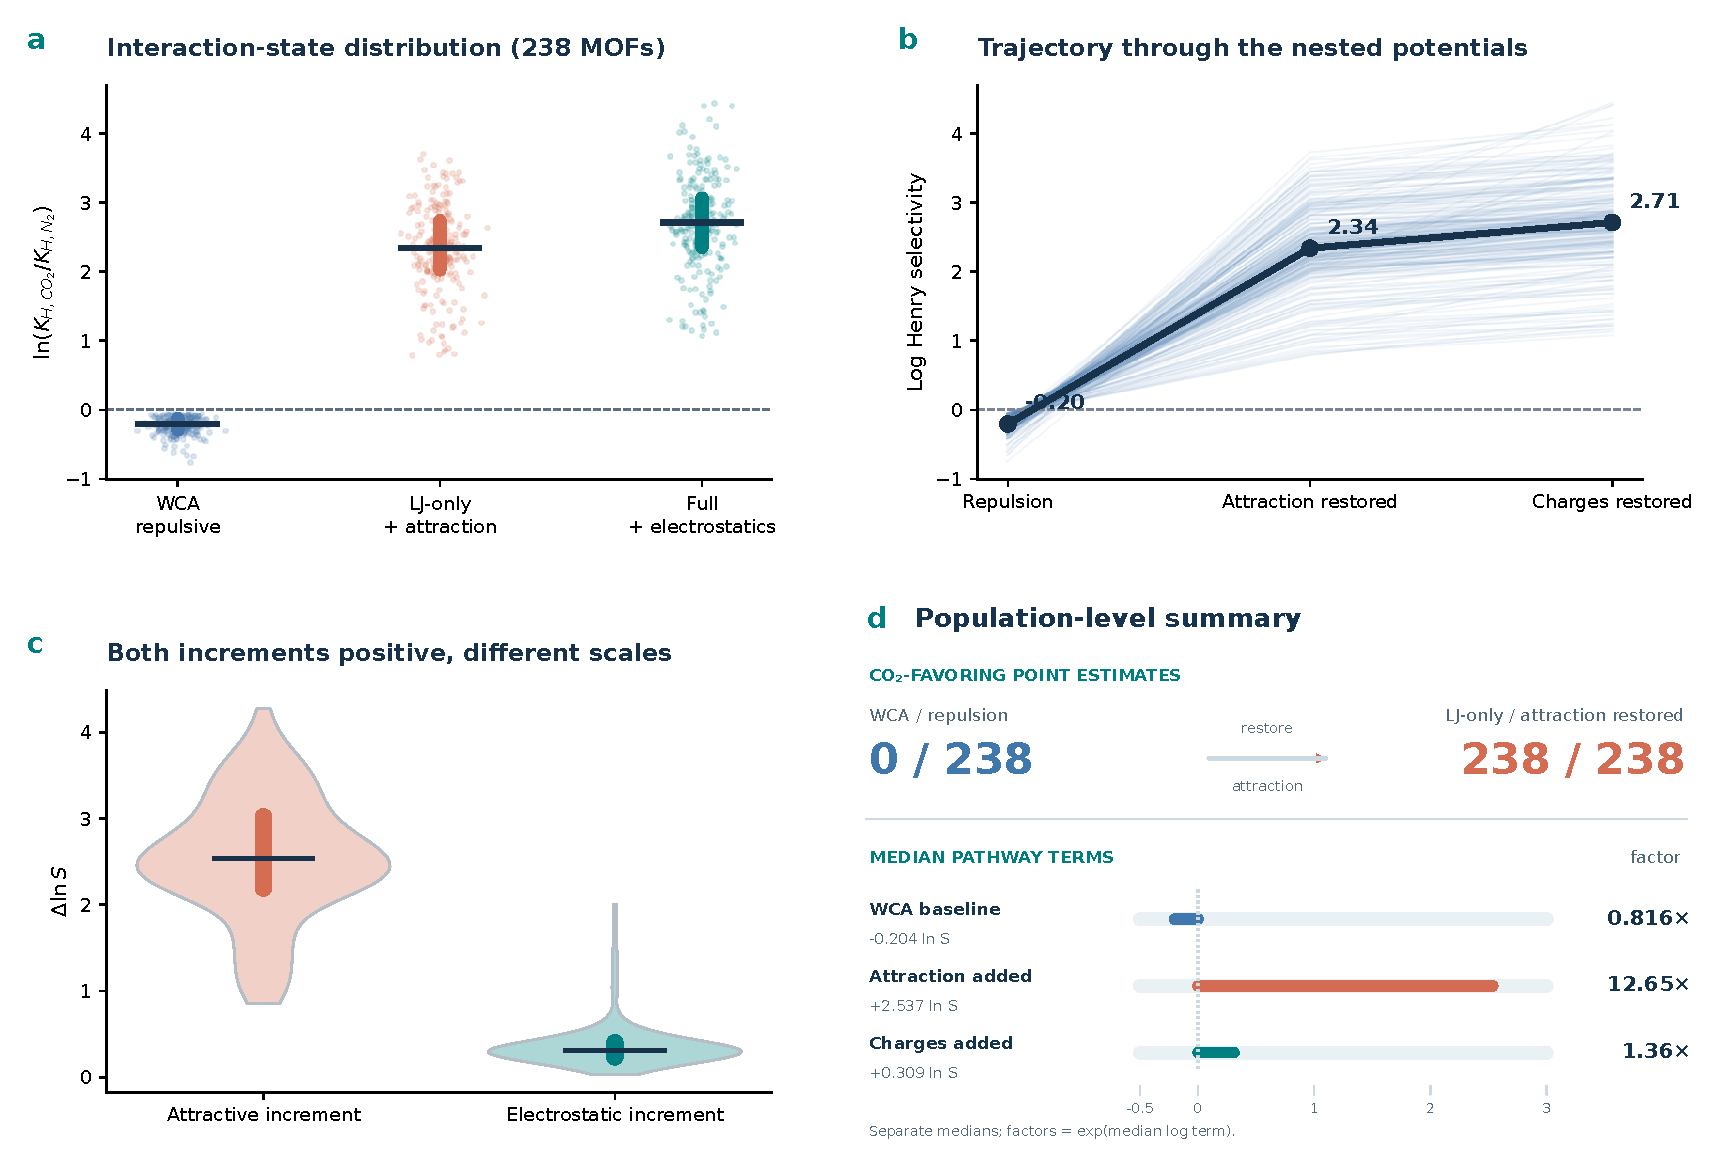
\includegraphics[width=\linewidth]{fig1_interaction_pathway.pdf}
\caption{\textbf{The nested interaction pathway reveals where CO$_2$ preference appears.} The WCA state provides the repulsive reference, the LJ-only state restores attractive Lennard--Jones interactions, and the full state additionally restores electrostatics. Across 238 MOFs the repulsive reference is N$_2$-favoring, the attractive increment is positive throughout the panel and reverses that preference, and electrostatics supplies an additional positive but heterogeneous increment.}
\label{fig:decomp}
\end{figure}

Uncertainty limits the wording of the universal-looking sign count. The WCA point estimate is negative in all 238 rows, but under an approximate point-estimate $\pm 1.96$ standard-error test, 19 individual upper bounds touch or exceed zero. Four WCA entries have standard errors above 0.10 log units. It is consequently appropriate to say that the archive displays an unambiguous \emph{population pattern} of N$_2$-favoring WCA estimates, but it would be stronger than the evidence to claim that each individual sign has independently cleared a 95\% confidence threshold. The supplementary precision plot makes the boundary visible.


\subsection{Electrostatics resolves different mechanisms}

Consistent with the established importance of charge assignments for CO$_2$ adsorption \cite{haldoupis2012charges,nazarian2016charges}, restoring electrostatics increases selectivity in every framework, with a median $\Delta\ln S_{\rm elec}=0.309$, equivalent to a 1.36-fold multiplicative contribution. Its magnitude, however, varies much more strongly from framework to framework than this positive sign alone suggests.

The attractive and electrostatic increments are only weakly associated across the population (Spearman $\rho=-0.089$; framework-bootstrap 95\% interval $-0.222$ to $0.050$; Figure~\ref{fig:map}). A framework that receives a large attractive enhancement does not necessarily receive a large electrostatic enhancement. This does not imply statistical independence; rather, once attractive interactions have established CO$_2$ preference, electrostatics introduces an additional dimension of framework-specific recognition.

The final selectivity is also mechanistically non-unique. Using the archived endpoint-matching rule, the closest 5\% of all 28,203 framework pairs in $|\ln S_{{\rm full},i}-\ln S_{{\rm full},j}|$ were retained (1,411 pairs; cutoff 0.0538) and then ranked by Euclidean distance in $(\Delta\ln S_{\rm attr},\Delta\ln S_{\rm elec})$. Within this endpoint-matched set, the median mechanism distance is 0.189 and the 95th percentile is 0.750. The strongest pair differs by only 0.016 in final $\ln S$ but has a mechanism distance of 2.585: its attractive/electrostatic increments are 2.211/2.001 versus 4.238/0.396. Thus nearly identical endpoint performance can be assembled from sharply different balances of attraction and electrostatics without altering the population-level sequential mechanism.

\begin{figure}[tbp]
\centering
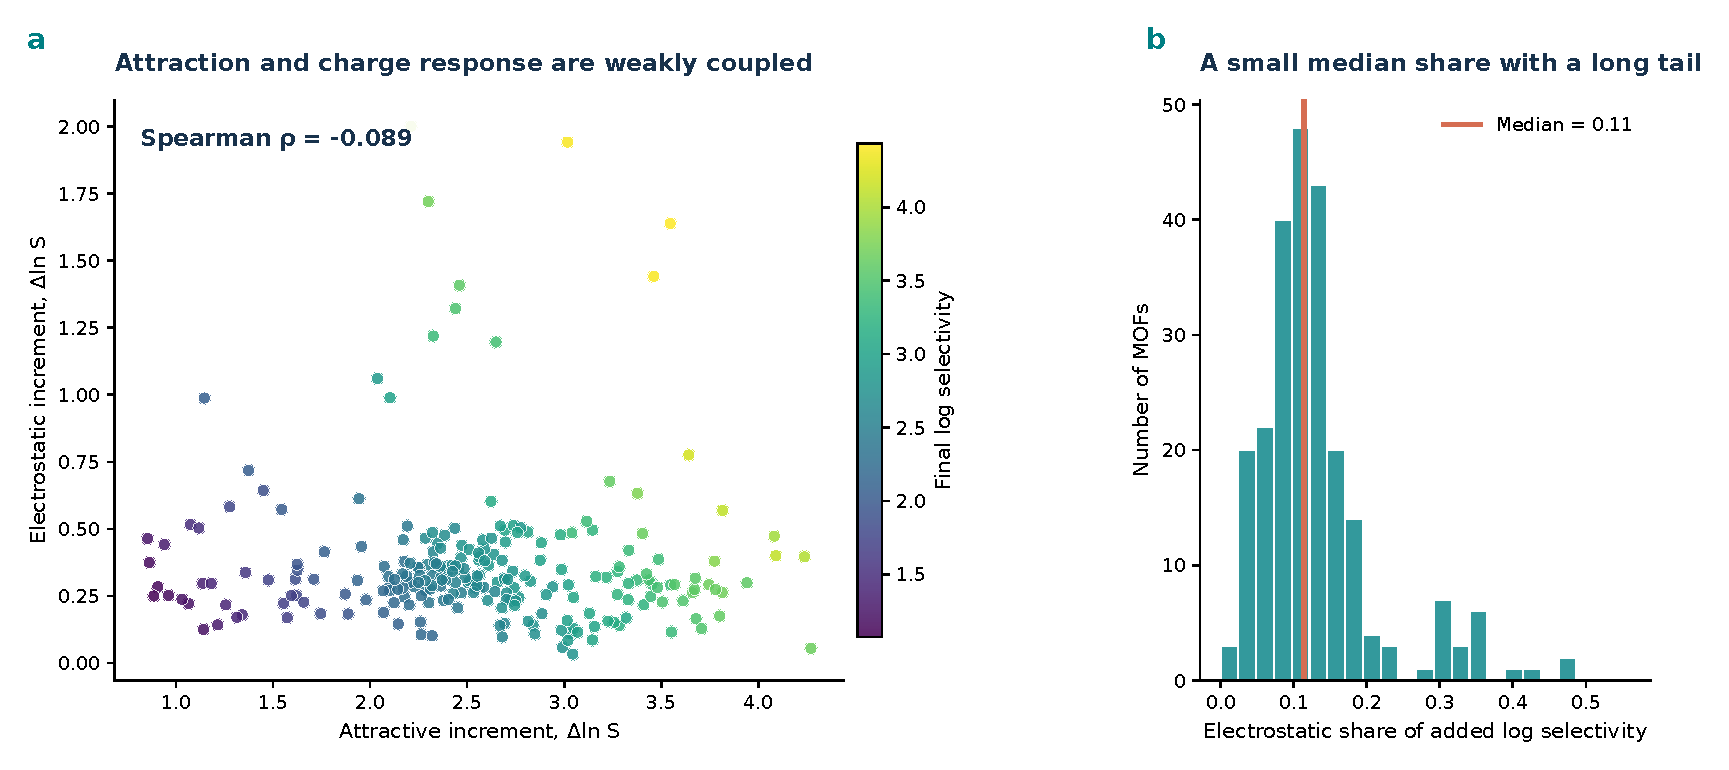
\includegraphics[width=\linewidth]{fig2_mechanism_diversity.pdf}
\caption{\textbf{Attractive and electrostatic changes retain distinct information.} (a) Continuous mechanism space for all 238 frameworks colored by final log-selectivity; attraction and electrostatics show a weak rank association. (b) Distribution of the share of the combined positive log-selectivity increment attributable to electrostatics. The endpoint-matched-pair analysis is reported in the text and Supporting Information, not depicted as a separate panel.} \label{fig:map}
\end{figure}

The two mechanisms of the highlighted endpoint-matched pair clarify why a ranking alone can mislead. One material reaches its final selectivity with an attractive increment of 2.211 followed by an electrostatic increment of 2.001, while the other uses 4.238 followed by 0.396. The roughly compensating increments leave their final selectivities only 0.016 log units apart. These are not interchangeable binding motifs, and a single final score has lost the information needed to distinguish them. The appropriate next experiment is to test whether selected mechanism-matched pairs respond differently to a predeclared perturbation, not merely to display more extreme pairs from the same dataset.


\subsection{Geometry predicts attraction more readily than electrostatics}

A critical alternative explanation is that the interaction coordinates merely restate conventional pore geometry, a useful screening basis in earlier work \cite{willems2012zeopp,fernandez2016geometry}. We therefore use 14 pre-simulation geometry descriptors as a control and ask how much information they contain about each stage of the decomposition.

Geometry-only ExtraTrees models give five-fold cross-validated $R^2=0.835$ for $\ln S_{\rm WCA}$ and $R^2=0.874$ for $\Delta\ln S_{\rm attr}$. Their mean absolute errors are 0.033 and 0.177, compared with median-predictor baselines of 0.093 and 0.549. Conventional pore geometry therefore contains substantial information about the repulsive reference and attractive confinement.

The electrostatic increment behaves differently. Geometry gives $R^2=0.188$, but its MAE of 0.146 is essentially identical to the median-predictor MAE of 0.147. Thus some population-level association remains, but geometry provides almost no practical improvement in absolute error for $\Delta\ln S_{\rm elec}$. The attraction--electrostatics predictability gap, $G=R^2_{\rm attr}-R^2_{\rm elec}$, is 0.686; a 5,000-resample framework bootstrap of the frozen out-of-fold predictions gives a 95\% interval of 0.560--0.905. Importantly, the same geometry descriptors still predict the final $\ln S_{\rm full}$ well ($R^2=0.845$; MAE 0.189 versus a 0.501 baseline). The role of this analysis is therefore mechanistic rather than predictive: the framework-to-framework variation in electrostatic recognition is not adequately reduced to the same pore-geometry information that captures the preceding stages. We do not interpret this as geometry being irrelevant to electrostatics.

Random cross-validation is also an interpolation test. It allows related topology and chemistry families to appear in both the training and held-out folds. Earlier family-grouped experiments in the archived version-2 analysis yielded poorer results for several electrostatic holdouts, but their model specifications are not identical to the frozen version-5 experiment and the numerical scores are not directly interchangeable. We retain these earlier outputs in the reproducibility materials as sensitivity evidence, while reporting the consistent version-5 analysis as the main control. A genuinely external test would require independent materials and a pre-registered feature-processing protocol.

This is why predicting the final selectivity is not the same as explaining it. The final log ratio includes a dominant attractive component that is already strongly associated with geometry. A model can learn that dominant signal and achieve a respectable endpoint $R^2$ while leaving much of the smaller, locally important electrostatic variation unresolved. For screening this may be satisfactory in an interpolative setting; for understanding the response to chemical substitution, partial-charge changes or out-of-family transfer it can be insufficient.

\begin{figure}[tbp]
\centering
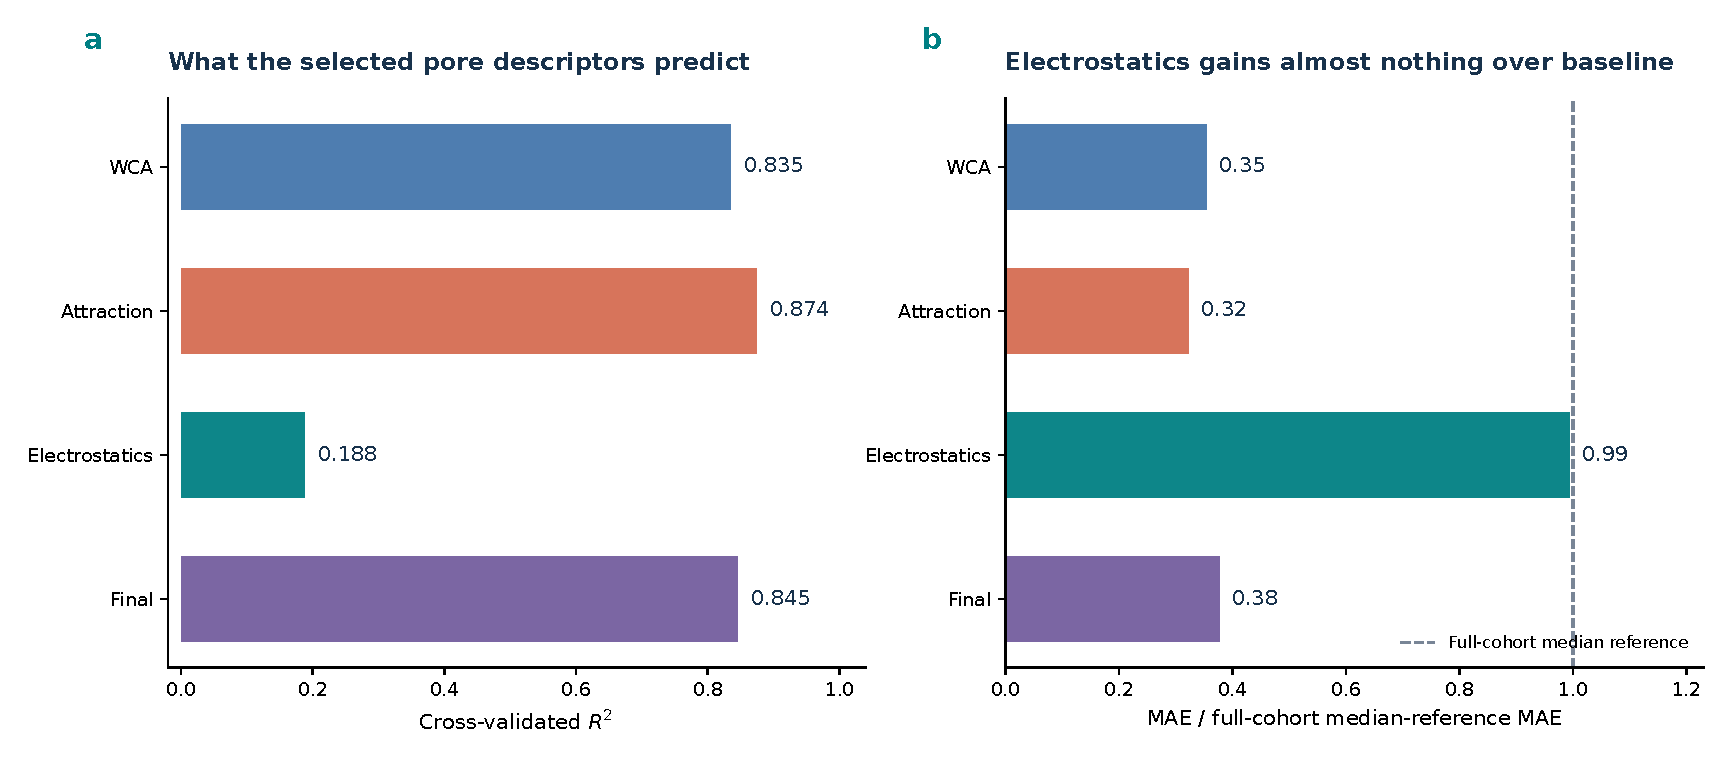
\includegraphics[width=\linewidth]{fig3_geometry_information.pdf}
\caption{\textbf{Pore geometry captures the attractive stage much more strongly than electrostatic variation.} (a) Five-fold out-of-fold $R^2$ of geometry-only models for the nested coordinates and final endpoint. (b) MAE normalized by the full-cohort median-reference MAE for all four targets; a value of one indicates no improvement over that descriptive reference. The bars and bootstrap are recomputed from restored saved final out-of-fold predictions; no model is refitted. The attraction--electrostatics $R^2$ gap is 0.686 with a framework-bootstrap 95\% interval of 0.560--0.905. This analysis is a mechanistic control rather than an ML benchmark.}
\label{fig:geometry}
\end{figure}


\subsection{Geometry-matched frameworks can differ in chemical recognition}

The retained illustrative electrostatic pair M029/M085 provides a local comparison for the population-level interpretation (Figure~\ref{fig:matched}). In the standardized nine-descriptor geometry space used for pair selection, the two structures are mutual nearest neighbors (distance 0.258). Their repulsive log-selectivities are nearly identical, $-0.201$ and $-0.198$, yet their electrostatic increments are 0.141 and 2.001, a difference of 1.860, corresponding to a 6.42-fold contrast in the multiplicative electrostatic contribution.

The global Henry coefficients identify which gas drives this divergence. Restoring electrostatics changes $\ln K_H$ for CO$_2$ by 0.162 in M029 and 2.032 in M085, whereas the N$_2$ changes are only 0.021 and 0.032. The between-framework difference is therefore 1.871 log units for CO$_2$ but only 0.011 for N$_2$: the stronger electrostatic recognition in M085 is overwhelmingly CO$_2$-driven.

Similarity in the nine matching descriptors does not establish chemical identity. The mutual nearest-neighbor relationship means that each member is the closest available entry to the other in that selected standardized descriptor space; it does not mean that every aperture, surface atom, charge distribution or adsorption-site orientation is identical. Identifier suffixes provide metadata labels but do not independently establish elemental composition or topology. We therefore base the pair comparison on its verified geometry coordinates and gas-resolved Henry responses, and reserve atomic or topological attribution for a structural analysis.

The gas-resolved values give the strongest evidence for where the contrast lies. For CO$_2$, the full-minus-LJ log-Henry response is 0.162 in M029 and 2.032 in M085. For N$_2$, the corresponding changes are only 0.021 and 0.032. The cross-material CO$_2$ difference is approximately 1.870 log units, while the N$_2$ difference is about 0.011. The resulting electrostatic-selectivity contrast is therefore primarily a CO$_2$ recognition effect in the evaluated model, not a similarly large redistribution of N$_2$ adsorption.

The next inference would be to assign this contrast to an atomic motif: a polar linker environment, a particular local coordination pattern, or a favorable orientation of the CO$_2$ quadrupole. That inference cannot be completed from the global Henry coefficients alone. The earlier manuscript contained visual spatial-field diagnostics, but the gridded values required to regenerate or quantitatively partition those maps were absent from the supplied archive. We have therefore not redrawn the earlier fields as if they were new simulation output. A chemically resolved follow-up would need a reproducible mapping between local host atoms and well-converged, normalized insertion-statistical weights.


\begin{figure}[tbp]
\centering
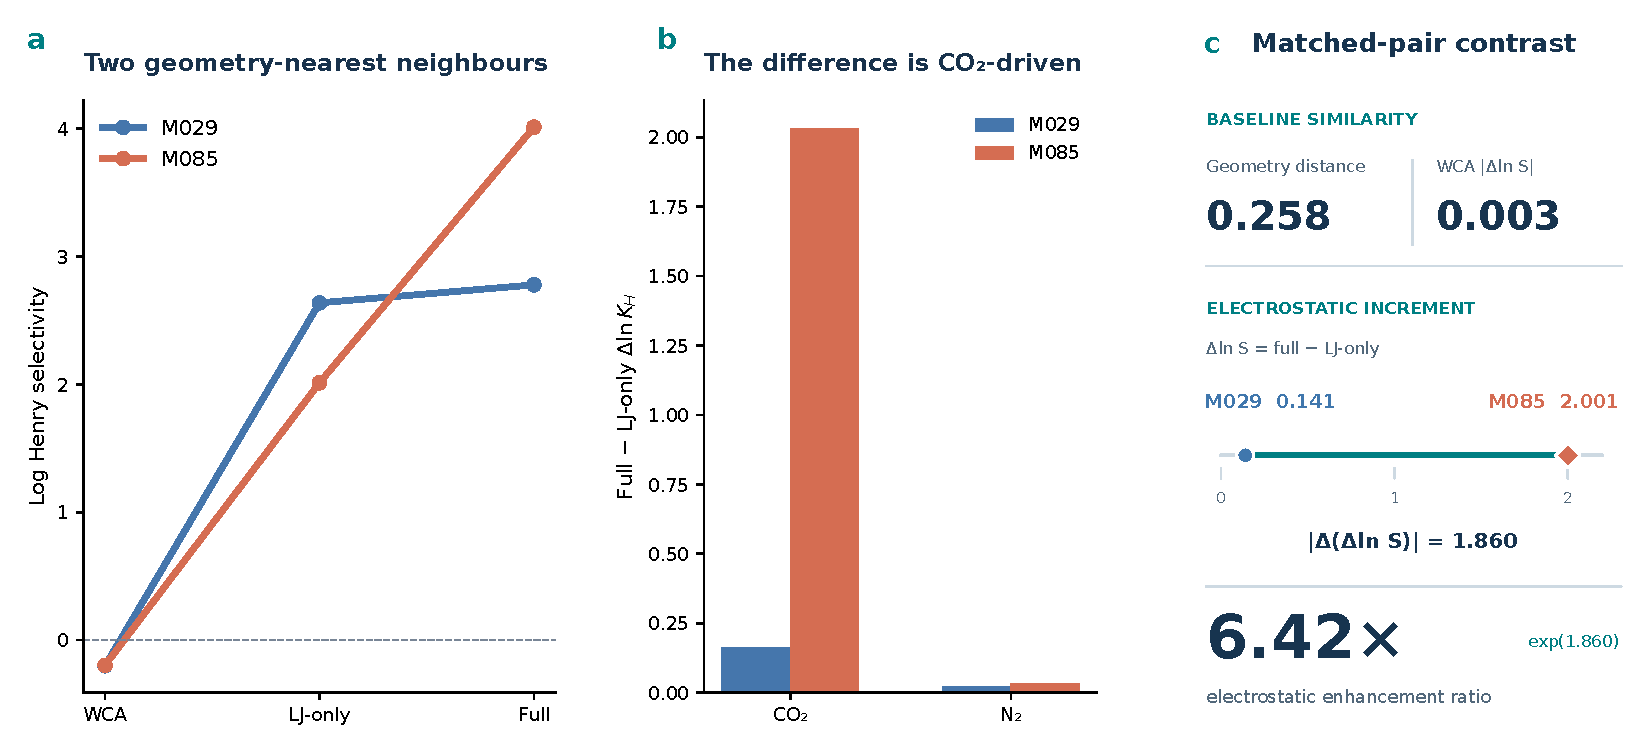
\includegraphics[width=\linewidth]{fig4_matched_contrast.pdf}
\caption{\textbf{A retained illustrative geometry-matched pair exhibits different electrostatic responses.} (a) Nested log-selectivity trajectories for M029 and M085, which are mutual nearest neighbors in the nine-descriptor matching space. (b) Full-minus-LJ log Henry increments for each gas. (c) Verified distance and scalar contrasts. These are retained examples from the restricted archived candidate procedure, not the optimal pair under the all-pair closest-2\% rule; the Supporting Information reports both rules separately.}
\label{fig:matched}
\end{figure}

\subsection{Consequences for candidate rankings}

The physical distinction between attraction and electrostatics has a direct consequence for candidate ordering. Restoring attraction reorganizes the population globally: WCA and LJ-only ranks have Spearman $\rho=-0.751$ and Kendall $\tau=-0.560$, with a median absolute displacement of 102 positions. Fully 89.5\% of frameworks move by at least 10\% of the 238-position range, 72.7\% move by at least 25\%, and 41.2\% move by at least 50\%. The top-10, top-25, and top-10\% sets have zero overlap between WCA and LJ-only rankings. The largest attraction-driven promotion and demotion are 234 and 226 positions.

Electrostatics acts differently. LJ-only and full ranks remain strongly correlated ($\rho=0.905$, $\tau=0.801$), with a median absolute displacement of only 9 positions. Only 17.2\%, 3.8\%, and 2.5\% of frameworks move by at least 10\%, 25\%, and 50\% of the ranking range, respectively; the top-10 overlap is 6/10 and the top-25 overlap is 18/25. Nevertheless, selected frameworks respond strongly, with promotions up to 175 positions. The ranking result is therefore a consequence of the mechanism identified above: attraction creates the global CO$_2$-selective landscape, whereas electrostatics mainly differentiates particular frameworks within it.

Given the limitations of equilibrium-ratio screening \cite{farmahini2020process}, from a materials-selection perspective the second transition is the more directly interpretable of the two. The WCA state has no physical attraction and is not a viable operational screening model, so its enormous rank changes upon restoring attraction should be read as a demonstration of mechanism. By contrast, the LJ-only-to-full comparison tells us how much candidate priority can change when electrostatic recognition is omitted from an otherwise attractive force field. Its high overall correlation coexists with striking local exceptions, precisely the kind of materials that a charge-free screening approximation might overlook.

\begin{figure}[tbp]
\centering
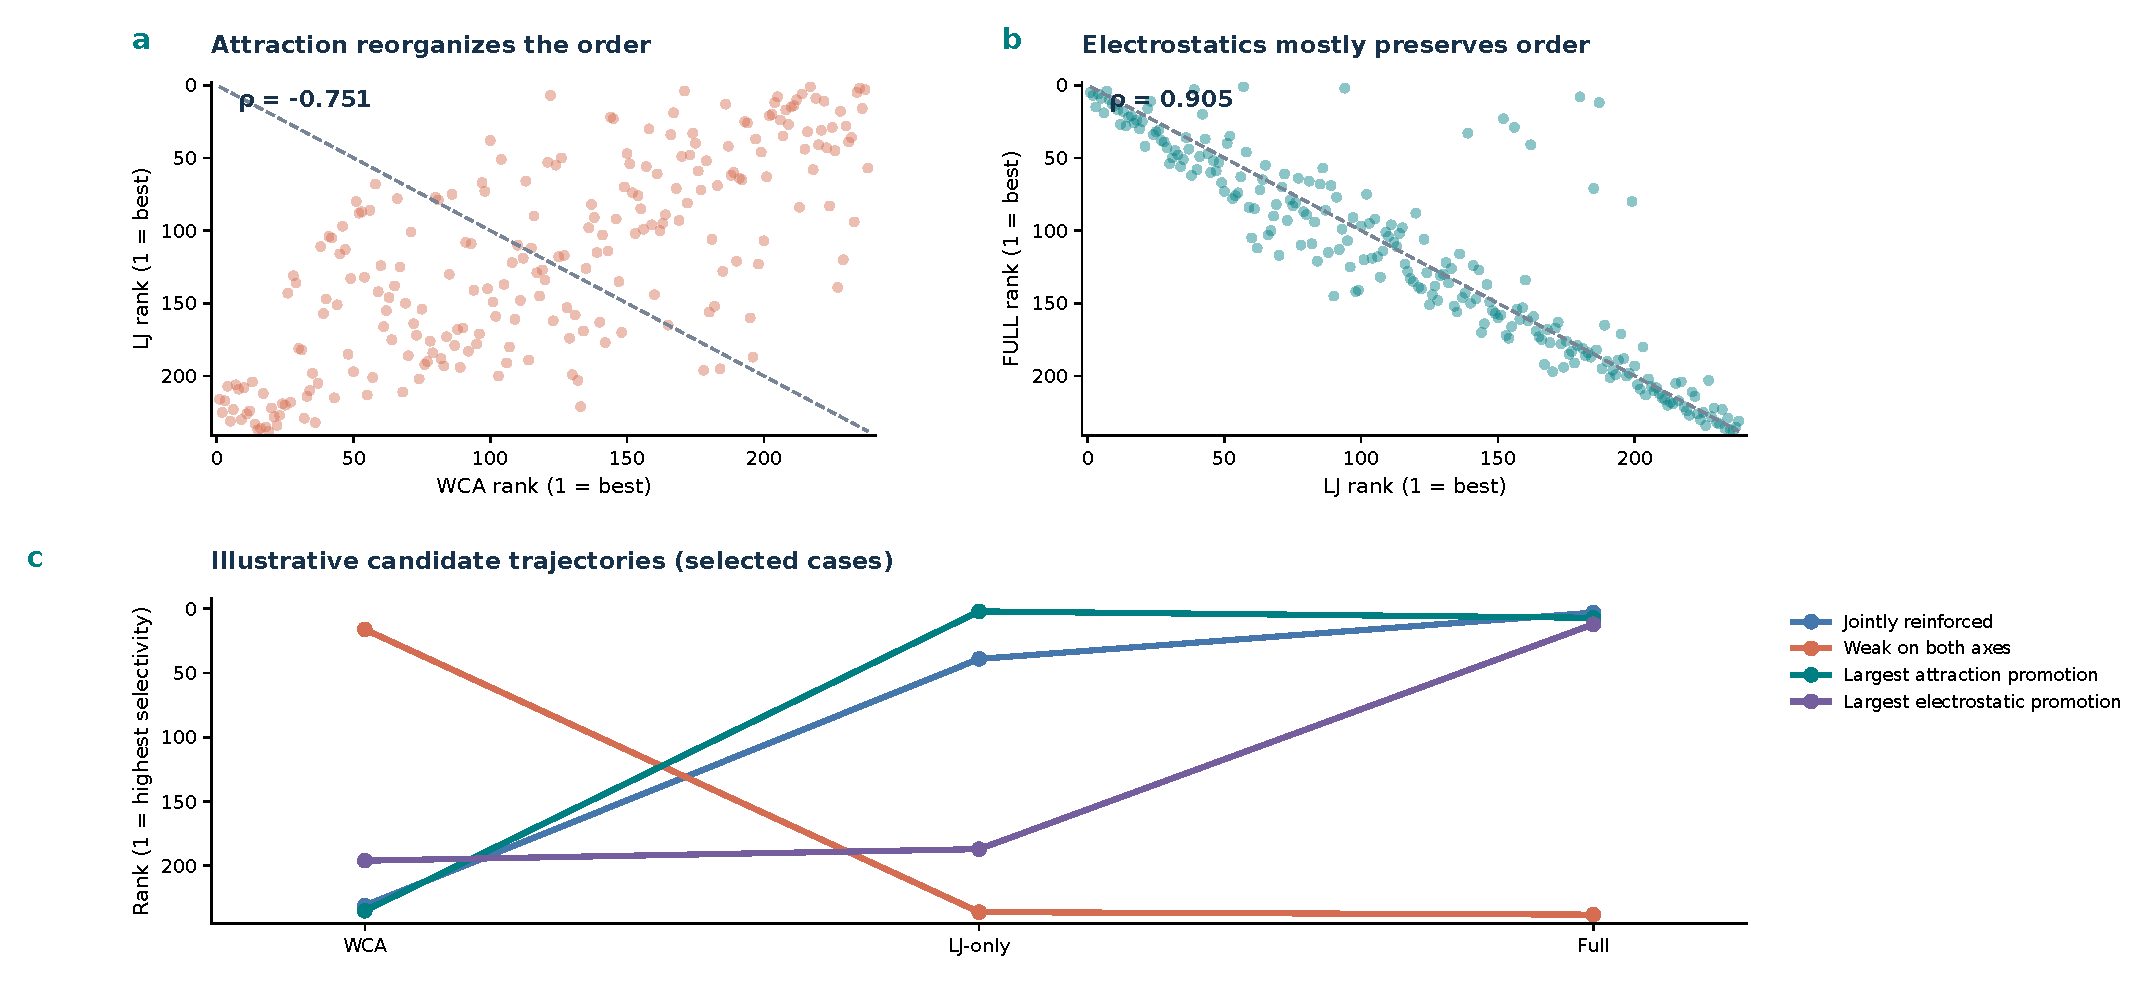
\includegraphics[width=\linewidth]{fig5_ranking_consequences.pdf}
\caption{\textbf{The interactions change material rankings in different ways.} (a,b) All 238 frameworks ranked by WCA versus LJ-only, then LJ-only versus full selectivity (1 = highest value). Dashed lines represent unchanged rank. (c) Four preselected illustrative trajectories obtained directly from the source table; they are examples, not representative frequencies.} \label{fig:ranks}
\end{figure}

The top-of-list effect is especially easy to interpret. Using the 24 highest-ranked entries as a fixed near-decile selection, the WCA and LJ-only rankings have \emph{zero} entries in common. Restoring the full LJ potential therefore changes not merely relative rank positions but the identity of every member of that selected shortlist. Because WCA is intentionally an incomplete reference potential, this should not be presented as the failure of a practical adsorption-screening technology. It shows how little the repulsive reference preserves the energetic ordering established by attractive confinement.

The LJ-only and complete-model top-24 lists instead share 17 entries. Thus seven entries enter and seven leave when electrostatics is included, even though the global Spearman rank correlation remains high. This is a useful way of stating what a high overall correlation can conceal. Broad population agreement does not guarantee stability precisely where a researcher is likely to spend the most time and money: the small candidate set sent to a more expensive calculation or synthesis campaign.


\subsection{Family dependence and scope}

Because the dataset contains a large dominant subgroup, we examined the two database identifier families separately as a transparent exploratory sensitivity analysis (Figure~\ref{fig:family}). In DB0-m15 ($n=210$), the median WCA, attractive, and electrostatic log increments are $-0.215$, 2.599, and 0.308. In DB0-m12 ($n=28$), the corresponding medians are $-0.087$, 1.755, and 0.313. Thus both subgroups retain the same qualitative direction of the three-stage mechanism, but the typical attractive amplification is markedly different. The smaller subgroup also contains fewer independent structures and should not carry the same inferential weight as the larger one.

The within-family correlation between the attractive and electrostatic increments is $-0.126$ in DB0-m15 and $+0.512$ in DB0-m12. These are descriptive Spearman estimates, not evidence that two independently sampled materials classes have different universal laws. Identifier family may coincide with topology, composition, or selection effects, and the group sizes are unequal. Still, the sign and magnitude difference demonstrates why a pooled correlation of $-0.089$ cannot be treated as an unconditional statement about every chemical subpopulation.

\begin{figure}[tbp]
\centering
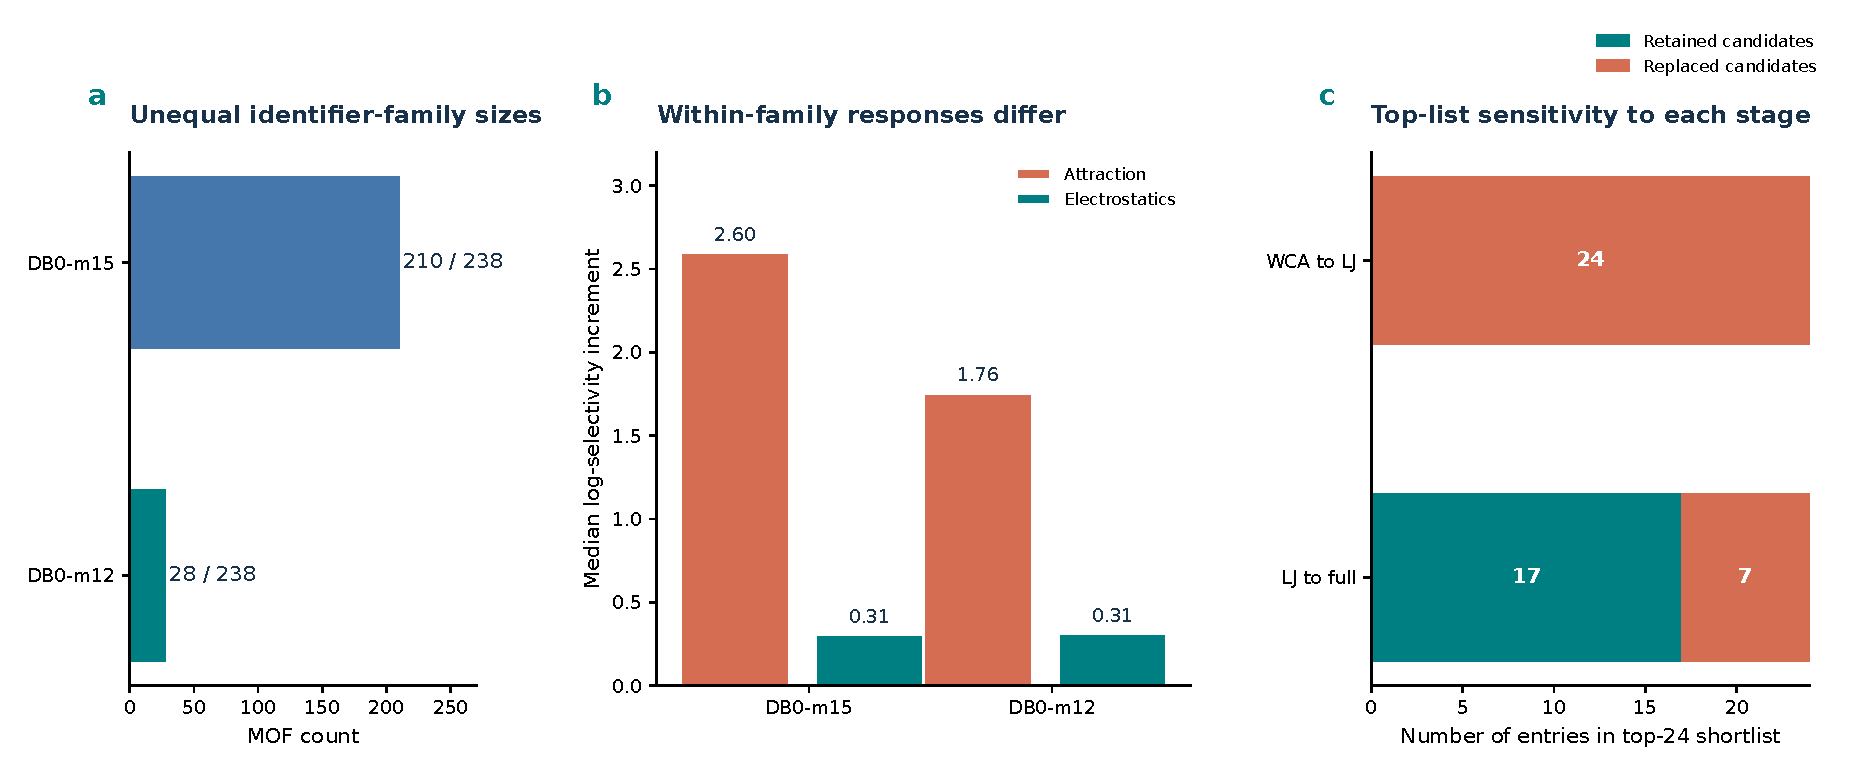
\includegraphics[width=\linewidth]{fig6_family_and_shortlist.pdf}
\caption{\textbf{Dataset concentration and shortlist sensitivity, calculated directly from the authoritative 238-MOF table.} (a) Analysis counts in the two DB0 identifier families. (b) Median attractive and electrostatic increments in each family; the unequal sizes should be kept in view. (c) Overlap of the top 24 selectivity-ranked candidates after restoring LJ attraction and then electrostatics. Overlaps are within-panel, point-estimate diagnostics and are not process-performance metrics.}
\label{fig:family}
\end{figure}

The results separate three questions that a single selectivity ratio merges: where discrimination first arises, how chemical recognition changes the magnitude of the preference, and whether the distinction matters for selecting candidates. The WCA-to-LJ rank reversal is mechanistic because the WCA reference is artificial, while the seven changes to the top-24 shortlist upon restoring electrostatics are more relevant to charge-free screening approximations. Neither result demonstrates separation-process superiority; process-scale rankings depend on loading, mixtures, transport, and cycle constraints \cite{farmahini2020process,farmahini2021screening}.

The decomposition is an intentionally ordered free-energy comparison, not an experimentally unique partition of interaction energies. The panel's limited chemical diversity, charge assignment, and rigid-framework assumption should therefore accompany every transfer claim. Independent-family simulations and alternative electrostatic models are needed to learn whether these fingerprints remain informative outside the present population.

\section{Conclusions}
A calculated CO$_2$/N$_2$ selectivity reports an endpoint, not the sequence of interactions that produced it. In the 238-framework panel studied here, all WCA reference point estimates favor N$_2$; restoring Lennard--Jones attraction reverses the preference throughout the panel, with a median 12.65-fold enhancement. Electrostatics adds a median 1.36-fold enhancement and produces marked differences between particular frameworks. The weak association between the attractive and electrostatic increments shows why identical final selectivities need not imply identical mechanisms.

The geometry control and matched-pair analysis support the same interpretation. Geometry captures much of the attractive variation but provides little improvement in absolute error for the electrostatic increment over a simple baseline. Two closely matched frameworks nevertheless exhibit a 6.42-fold contrast in electrostatic enhancement, driven primarily by CO$_2$. Restoring charges also changes seven members of the LJ-only top-24 shortlist.

These conclusions apply to a chemically concentrated, rigid-framework panel at infinite dilution and to a declared switching path. They do not establish force-field-independent decomposition or real-process superiority. The practical lesson is narrower and useful: when materials are selected from a single computed ratio, information about chemical recognition can be lost. Testing the same interaction map on independent chemistry families and under finite-loading conditions would determine whether that information can improve decisions beyond the present dataset.
\section*{Supporting Information}
Extended methods, force-field details, statistical precision checks, family and shortlist analyses, supplementary figures, and a source-data inventory (PDF); tabulated analysis data and figure-generation code (ZIP).

\section*{Data Availability}
The framework-level results, matching final saved OOF predictions, statistical analyses, explicit figure sources, code and provenance manifests are supplied in the companion repository, \url{https://github.com/alimardani76/bundle_molsim}. The unchanged 238-framework cohort supports regeneration of the numerical results and figures without model refitting. The original structural and per-job simulation inputs are not supplied as a complete runnable set; fresh molecular simulation is therefore outside the reproducibility claim of this release.
\bibliography{references}
\end{document}
